\upaper{32}{The Evolution of Local Universes}
\uminitoc{Physical Emergence of Universes}
\uminitoc{Universe Organization}
\uminitoc{The Evolutionary Idea}
\uminitoc{God’s Relation to a Local Universe}
\uminitoc{The Eternal and Divine Purpose}
\author{Mighty Messenger}
\vs p032 0:1 A local universe is the handiwork of a Creator Son of the Paradise order of Michael. It comprises 100 constellations, each embracing 100 systems of inhabited worlds. Each system will eventually contain approximately 1,000 inhabited spheres.
\vs p032 0:2 These universes of time and space are all evolutionary. The creative plan of the Paradise Michaels always proceeds along the path of gradual evolvement and progressive development of the physical, intellectual, and spiritual natures and capacities of the manifold creatures who inhabit the varied orders of spheres comprising such a local universe.
\vs p032 0:3 Urantia belongs to a local universe whose sovereign is the God\hyp{}man of Nebadon, Jesus of Nazareth and Michael of Salvington. And all of Michael’s plans for this local universe were fully approved by the Paradise Trinity before he ever embarked upon the supreme adventure of space.
\vs p032 0:4 The Sons of God may choose the realms of their creator activities, but these material creations were originally projected and planned by the Paradise Architects of the Master Universe.
\usection{Physical Emergence of Universes}
\vs p032 1:1 The preuniverse manipulations of space\hyp{}force and the primordial energies are the work of the Paradise Master Force Organizers; but in the superuniverse domains, when emergent energy becomes responsive to local or linear gravity, they retire in favour of the power directors of the superuniverse concerned.
\vs p032 1:2 These power directors function alone in the prematerial and postforce phases of a local universe creation. There is no opportunity for a Creator Son to begin universe organization until the power directors have effected the mobilization of the space\hyp{}energies sufficiently to provide a material foundation --- literal suns and material spheres --- for the emerging universe.
\vs p032 1:3 \pc The local universes are all approximately of the same energy potential, though they differ greatly in physical dimensions and may vary in visible\hyp{}matter content from time to time. The power charge and potential\hyp{}matter endowment of a local universe are determined by the manipulations of the power directors and their predecessors as well as by the Creator Son’s activities and by the endowment of the inherent physical control possessed by his creative associate.
\vs p032 1:4 The energy charge of a local universe is approximately\fnst{\textbf{approximately}, In \bibref[15:4.6]{p015 4:6} we are told this is \bibemph{exactly} so, not \bibemph{approximately}. The only apparent difference is that there it refers to the \bibemph{energy charge}, whereas here to the \bibemph{force endowment} of a superuniverse.} 1/100,000\ts{th} of the force endowment of its superuniverse. In the case of Nebadon, your local universe, the mass materialization is a trifle less. Physically speaking, Nebadon possesses all of the physical endowment of energy and matter that may be found in any of the Orvonton local creations. The only physical limitation upon the developmental expansion of the Nebadon universe consists in the quantitative charge of space\hyp{}energy held captive by the gravity control of the associated powers and personalities of the combined universe mechanism.
\vs p032 1:5 \pc When energy\hyp{}matter has attained a certain stage in mass materialization, a Paradise Creator Son appears upon the scene, accompanied by a Creative Daughter of the Infinite Spirit. Simultaneously with the arrival of the Creator Son, work is begun upon the architectural sphere which is to become the headquarters world of the projected local universe. For long ages such a local creation evolves, suns become stabilized, planets form and swing into their orbits, while the work of creating the architectural worlds which are to serve as constellation headquarters and system capitals continues.
\usection{Universe Organization}
\vs p032 2:1 The Creator Sons are preceded in universe organization by the power directors and other beings originating in the Third Source and Centre. From the energies of space, thus previously organized, Michael, your Creator Son, established the inhabited realms of the universe of Nebadon and ever since has been painstakingly devoted to their administration. From pre\hyp{}existent energy these divine Sons materialize visible matter, project living creatures, and with the co\hyp{}operation of the universe presence of the Infinite Spirit, create a diverse retinue of spirit personalities.
\vs p032 2:2 These power directors and energy controllers who long preceded the Creator Son in the preliminary physical work of universe organization later serve in magnificent liaison with this Universe Son, forever remaining in associated control of those energies which they originally organized and circuitized. On Salvington there now function the same 100 power centres who co\hyp{}operated with your Creator Son in the original formation of this local universe.
\vs p032 2:3 \pc The first completed act of physical creation in Nebadon consisted in the organization of the headquarters world, the architectural sphere of Salvington, with its satellites. From the time of the initial moves of the power centres and physical controllers to the arrival of the living staff on the completed spheres of Salvington, there intervened a little over one billion years of your present planetary time. The construction of Salvington was immediately followed by the creation of the 100 headquarters worlds of the projected constellations and the 10,000 headquarters spheres of the projected local systems of planetary control and administration, together with their architectural satellites. Such architectural worlds are designed to accommodate both physical and spiritual personalities as well as the intervening morontia or transition stages of being.
\vs p032 2:4 Salvington, the headquarters of Nebadon, is situated at the exact energy\hyp{}mass centre of the local universe. But your local universe is not a single astronomic system, though a large system does exist at its physical centre.
\vs p032 2:5 Salvington is the personal headquarters of Michael of Nebadon, but he will not always be found there. While the smooth functioning of your local universe no longer requires the fixed presence of the Creator Son at the capital sphere, this was not true of the earlier epochs of physical organization. A Creator Son is unable to leave his headquarters world until such a time as gravity stabilization of the realm has been effected through the materialization of sufficient energy to enable the various circuits and systems to counterbalance one another by mutual material attraction.
\vs p032 2:6 \pc Presently, the physical plan of a universe is completed, and the Creator Son, in association with the Creative Spirit, projects his plan of life creation; whereupon does this representation of the Infinite Spirit begin her universe function as a distinct creative personality. When this first creative act is formulated and executed, there springs into being the Bright and Morning Star, the personification of this initial creative concept of identity and ideal of divinity. This is the chief executive of the universe, the personal associate of the Creator Son, one like him in all aspects of character, though markedly limited in the attributes of divinity.
\vs p032 2:7 And now that the right\hyp{}hand helper and chief executive of the Creator Son has been provided, there ensues the bringing into existence of a vast and wonderful array of diverse creatures. The sons and daughters of the local universe are forthcoming, and soon thereafter the government of such a creation is provided, extending from the supreme councils of the universe to the fathers of the constellations and the sovereigns of the local systems --- the aggregations of those worlds which are designed subsequently to become the homes of the varied mortal races of will creatures; and each of these worlds will be presided over by a Planetary Prince.
\vs p032 2:8 And then, when such a universe has been so completely organized and so repletely manned, does the Creator Son enter into the Father’s proposal to create mortal man in their divine image.
\vs p032 2:9 \pc The organization of planetary abodes is still progressing in Nebadon, for this universe is, indeed, a young cluster in the starry and planetary realms of Orvonton. At the last registry there were 3,840,101 inhabited planets in Nebadon, and Satania, the local system of your world, is fairly typical of other systems.\tunemarkup{pictures}{\begin{figure}[H]\centering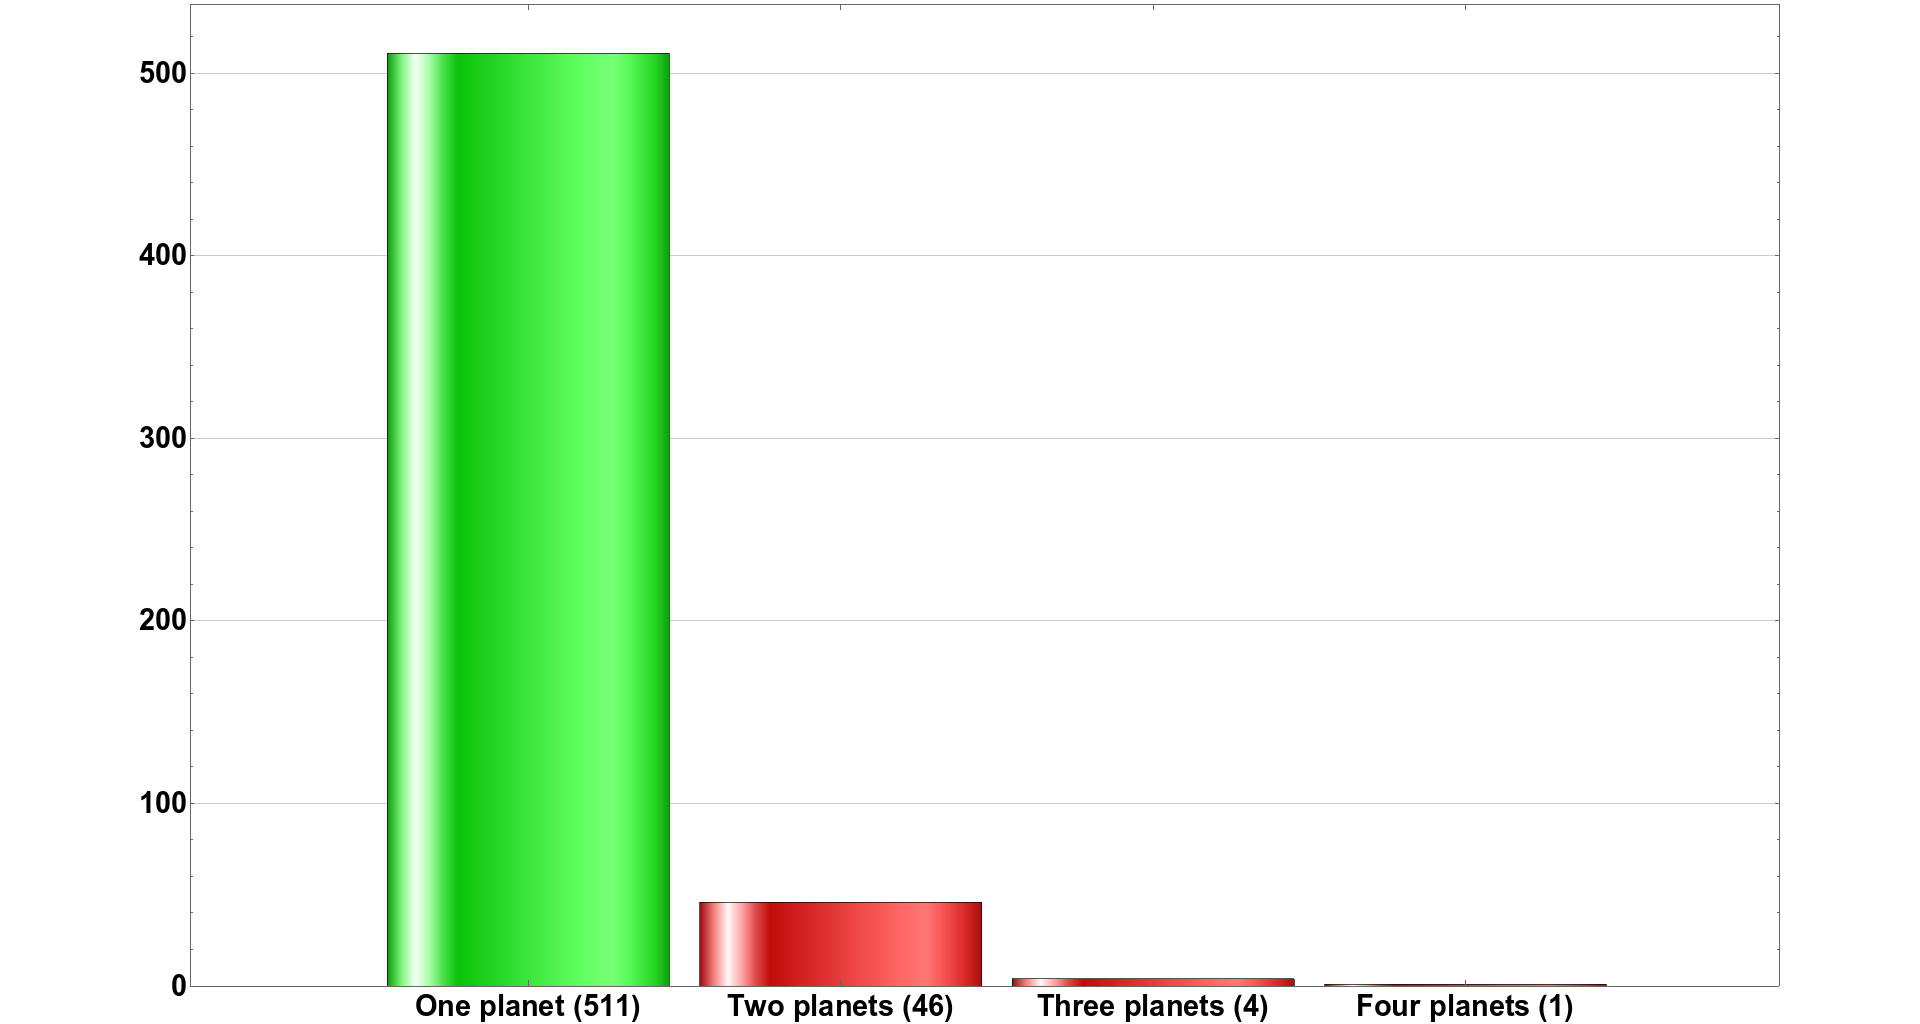
\includegraphics[width=\columnwidth]{images/planet-systems.png}\caption{Distribution of 562 Systems by Number of Planets, presumed Solar System type (``One planet'') is marked with green.}\end{figure}}
\vs p032 2:10 Satania is not a uniform physical system, a single astronomic unit or organization. Its 619 inhabited worlds are located in over 500 different physical systems\fnst{\textbf{over 500 \ldots\ systems}, More precisely: 562 systems, of which 511 are with 1, 46 with 2, 4 with 3 and 1 with 4 inhabited planets.}. Only 5 have more than 2 inhabited worlds, and of these only 1 has 4 peopled planets, while there are 46 having 2 inhabited worlds.
\vs p032 2:11 The Satania system of inhabited worlds is far removed from Uversa and that great sun cluster which functions as the physical or astronomic centre of the seventh superuniverse. From Jerusem, the headquarters of Satania, it is over 200,000 light\hyp{}years to the physical centre of the superuniverse of Orvonton, far, far away in the dense diameter of the Milky Way. Satania is on the periphery of the local universe, and Nebadon is now well out towards the edge of Orvonton. From the outermost system of inhabited worlds to the centre of the superuniverse is a trifle less than 250,000 light\hyp{}years\fnst{\textbf{250,000 light\hyp{}years}, This implies that the present estimate of the size of Milky Way galaxy (100,000\,ly) is at least five times lower than the actual size thereof.}.
\vs p032 2:12 The universe of Nebadon now swings far to the south and east in the superuniverse circuit of Orvonton. The nearest neighbouring universes are: Avalon\fnst{\textbf{Avalon}, This word occurs 5 times in the Urantia Papers (\bibref[38:5.1]{p038 5:1}, \bibref[66:2.7]{p066 2:7}, \bibref[67:6.5]{p067 6:5} and \bibref[77:2.6]{p077 2:6}). The word ``Avalon'' first appears in Geoffrey of Monmouth's historical account \bibemph{Historia Regum Britanni\ae} (``The History of the Kings of Britain'', c.~1136) as the place where King Arthur's sword Excalibur (Caliburnus) was forged and later where Arthur was taken to recover from his wounds after the Battle of Camlann --- his final battle (and the word ``Camlann'' signifying ``crooked''). The island was ruled by the enchantress Morgan le Fay and her eight sisters, all of them skilled in the healing arts. In Latin it was called \bibemph{Insula Avallonis} in the \bibemph{Historia}. In the later \bibemph{Vita Merlini} (``The Life of Merlin'', c.~1150) he called it \bibemph{Insula Pomorum} the ``isle of apples''. The name is generally considered to be of Welsh origin (though an Old Cornish or Old Breton origin is also possible), derived from Old Welsh \bibemph{abal}, ``apple'', or \bibemph{aball}, ``apple tree'' (in later Middle Welsh spelled \bibemph{aval, avall;} now Modern Welsh \bibemph{afal, afall}). Sir John Rhys, however (\bibemph{Studies in the Arthurian Legend}, 1891), linked the name Avalon with that of Aballach, a dark Celtic divinity and places Avalon at the west coast in Cornwall. Malory identifies Avalon with Glastonbury in Somerset, and this may be connected with Celtic legends about an ``isle of glass'' inhabited by deceased heroes.}, Henselon, Sanselon, Portalon, Wolvering, Fanoving, and Alvoring.
\vs p032 2:13 \pc But the evolution of a local universe is a long narrative. Papers dealing with the superuniverse introduce this subject, those of this section, treating of the local creations, continue it, while those to follow, touching upon the history and destiny of Urantia, complete the story. But you can adequately comprehend the destiny of the mortals of such a local creation only by a perusal of the narratives of the life and teachings of your Creator Son as he once lived the life of man, in the likeness of mortal flesh, on your own evolutionary world.
\usection{The Evolutionary Idea}
\vs p032 3:1 The only creation that is perfectly settled is Havona, the central universe, which was made directly by the thought of the Universal Father and the word of the Eternal Son. Havona is an existential, perfect, and replete universe, surrounding the home of the eternal Deities, the centre of all things. The creations of the seven superuniverses are finite, evolutionary, and consistently progressive.
\vs p032 3:2 The physical systems of time and space are all evolutionary in origin. They are not even physically stabilized until they are swung into the settled circuits of their superuniverses. Neither is a local universe settled in light and life until its physical possibilities of expansion and development have been exhausted, and until the spiritual status of all its inhabited worlds has been forever settled and stabilized.
\vs p032 3:3 Except in the central universe, perfection is a progressive attainment. In the central creation we have a pattern of perfection, but all other realms must attain that perfection by the methods established for the advancement of those particular worlds or universes. And an almost infinite variety characterizes the plans of the Creator Sons for organizing, evolving, disciplining, and settling their respective local universes.
\vs p032 3:4 \pc With the exception of the deity presence of the Father, every local universe is, in a certain sense, a duplication of the administrative organization of the central or pattern creation. Although the Universal Father is personally present in the residential universe, he does not indwell the minds of the beings originating in that universe as he does literally dwell with the souls of the mortals of time and space. There seems to be an all\hyp{}wise compensation in the adjustment and regulation of the spiritual affairs of the far\hyp{}flung creation. In the central universe the Father is personally present as such but absent in the minds of the children of that perfect creation; in the universes of space the Father is absent in person, being represented by his Sovereign Sons, while he is intimately present in the minds of his mortal children, being spiritually represented by the prepersonal presence of the Mystery Monitors that reside in the minds of these will creatures.
\vs p032 3:5 On the headquarters of a local universe there reside all those creator and creative personalities who represent self\hyp{}contained authority and administrative autonomy except the personal presence of the Universal Father. In the local universe there are to be found something of everyone and someone of almost every class of intelligent beings existing in the central universe except the Universal Father. Although the Universal Father is not personally present in a local universe, he is personally represented by its Creator Son, sometime vicegerent of God and subsequently supreme and sovereign ruler in his own right.
\vs p032 3:6 The farther down the scale of life we go, the more difficult it becomes to locate, with the eye of faith, the invisible Father. The lower creatures --- and sometimes even the higher personalities --- find it difficult always to envisage the Universal Father in his Creator Sons. And so, pending the time of their spiritual exaltation, when perfection of development will enable them to see God in person, they grow weary in progression, entertain spiritual doubts, stumble into confusion, and thus isolate themselves from the progressive spiritual aims of their time and universe. In this way they lose the ability to see the Father when beholding the Creator Son. The surest safeguard for the creature throughout the long struggle to attain the Father, during this time when inherent conditions make such attainment impossible, is tenaciously to hold on to the truth\hyp{}fact of the Father’s presence in his Sons. Literally and figuratively, spiritually and personally, the Father and the Sons are one. It is a fact: He who has seen a Creator Son has seen the Father.
\vs p032 3:7 \pc The personalities of a given universe are settled and dependable, at the start, only in accordance with their degree of kinship to Deity. When creature origin departs sufficiently far from the original and divine Sources, whether we are dealing with the Sons of God or the creatures of ministry belonging to the Infinite Spirit, there is an increase in the possibility of disharmony, confusion, and sometimes rebellion --- sin.
\vs p032 3:8 \pc Excepting perfect beings of Deity origin, all will creatures in the superuniverses are of evolutionary nature, beginning in lowly estate and climbing ever upward, in reality inward. Even highly spiritual personalities continue to ascend the scale of life by progressive translations from life to life and from sphere to sphere. And in the case of those who entertain the Mystery Monitors, there is indeed no limit to the possible heights of their spiritual ascent and universe attainment.
\vs p032 3:9 The perfection of the creatures of time, when finally\tunemarkup{pgnexus10}{\linebreak} achieved, is wholly an acquirement, a bona fide personality possession. While the elements of grace are freely admixed, nevertheless, the creature attainments are the result of individual effort and actual living, personality reaction to the existing environment.
\vs p032 3:10 The fact of animal evolutionary origin does not attach stigma to any personality in the sight of the universe as that is the exclusive method of producing one of the two basic types of finite intelligent will creatures. When the heights of perfection and eternity are attained, all the more honour to those who began at the bottom and joyfully climbed the ladder of life, round by round, and who, when they do reach the heights of glory, will have gained a personal experience which embodies an actual knowledge of every phase of life from the bottom to the top.
\vs p032 3:11 In all this is shown the wisdom of the Creators. It would be just as easy for the Universal Father to make all mortals perfect beings, to impart perfection by his divine word. But that would deprive them of the wonderful experience of the adventure and training associated with the long and gradual inward climb, an experience to be had only by those who are so fortunate as to begin at the very bottom of living existence.
\vs p032 3:12 In the universes encircling Havona there are provided only a sufficient number of perfect creatures to meet the need for pattern teacher guides for those who are ascending the evolutionary scale of life. The experiential nature of the evolutionary type of personality is the natural cosmic complement of the ever\hyp{}perfect natures of the Paradise\hyp{}Havona creatures. In reality, both perfect and perfected creatures are incomplete as regards finite totality. But in the complemental association of the existentially perfect creatures of the Paradise\hyp{}Havona system with the experientially perfected finaliters ascending from the evolutionary universes, both types find release from inherent limitations and thus may conjointly attempt to reach the sublime heights of the ultimate of creature status.
\vs p032 3:13 These creature transactions are the universe repercussions of actions and reactions within the Sevenfold Deity, wherein the eternal divinity of the Paradise Trinity is conjoined with the evolving divinity of the Supreme Creators of the time\hyp{}space universes in, by, and through the power\hyp{}actualizing Deity of the Supreme Being.
\vs p032 3:14 The divinely perfect creature and the evolutionary perfected creature are equal in degree of divinity potential, but they differ in kind. Each must depend on the other to attain supremacy of service. The evolutionary superuniverses depend on perfect Havona to provide the final training for their ascending citizens, but so does the perfect central universe require the existence of the perfecting superuniverses to provide for the full development of its descending inhabitants.
\vs p032 3:15 The two prime manifestations of finite reality, innate perfection and evolved perfection, be they personalities or universes, are co\hyp{}ordinate, dependent, and integrated. Each requires the other to achieve completion of function, service, and destiny.
\usection{God’s Relation to a Local Universe}
\vs p032 4:1 Do not entertain the idea that, since the Universal Father has delegated so much of himself and his power to others, he is a silent or inactive member of the Deity partnership. Aside from personality domains and Adjuster bestowal, he is apparently the least active of the Paradise Deities in that he allows his Deity co\hyp{}ordinates, his Sons, and numerous created intelligences to perform so much in the carrying out of his eternal purpose. He is the silent member of the creative trio only in that he never does aught which any of his co\hyp{}ordinate or subordinate associates can do.
\vs p032 4:2 God has full understanding of the need of every intelligent creature for function and experience, and therefore, in every situation, be it concerned with the destiny of a universe or the welfare of the humblest of his creatures, God retires from activity in favour of the galaxy of creature and Creator personalities who inherently intervene between himself and any given universe situation or creative event. But notwithstanding this retirement, this exhibition of infinite co\hyp{}ordination, there is on God’s part an actual, literal, and personal participation in these events by and through these ordained agencies and personalities. The Father is working in and through all these channels for the welfare of all his far\hyp{}flung creation.
\vs p032 4:3 \pc As regards the policies, conduct, and administration of a local universe, the Universal Father acts in the person of his Creator Son. In the interrelationships of the Sons of God, in the group associations of the personalities of origin in the Third Source and Centre, or in the relationship between any other creatures, such as human beings --- as concerns such associations the Universal Father never intervenes. The law of the Creator Son, the rule of the Constellation Fathers, the System Sovereigns, and the Planetary Princes --- the ordained policies and procedures for that universe --- always prevail. There is no division of authority; never is there a cross working of divine power and purpose. The Deities are in perfect and eternal unanimity.
\vs p032 4:4 The Creator Son rules supreme in all matters of ethical associations, the relations of any division of creatures to any other class of creatures or of two or more individuals within any given group; but such a plan does not mean that the Universal Father may not in his own way intervene and do aught that pleases the divine mind with any \bibemph{individual creature} throughout all creation, as pertains to that individual’s present status or future prospects and as concerns the Father’s eternal plan and infinite purpose.
\vs p032 4:5 \pc In the mortal will creatures the Father is actually present in the indwelling Adjuster, a fragment of his prepersonal spirit; and the Father is also the source of the personality of such a mortal will creature.
\vs p032 4:6 \pc These Thought Adjusters, the bestowals of the Universal Father, are comparatively isolated; they indwell human minds but have no discernible connection with the ethical affairs of a local creation. They are not directly co\hyp{}ordinated with the seraphic service nor with the administration of systems, constellations, or a local universe, not even with the rule of a Creator Son, whose will is the supreme law of his universe.
\vs p032 4:7 The indwelling Adjusters are one of God’s separate but unified modes of contact with the creatures of his all but infinite creation. Thus does he who is invisible to mortal man manifest his presence, and could he do so, he would show himself to us in still other ways, but such further revelation is not divinely possible.
\vs p032 4:8 We can see and understand the mechanism whereby the Sons enjoy intimate and complete knowledge regarding the universes of their jurisdiction; but we cannot fully comprehend the methods whereby God is so fully and personally conversant with the details of the universe of universes, although we at least can recognize the avenue whereby the Universal Father can receive information regarding, and manifest his presence to, the beings of his immense creation. Through the personality circuit the Father is cognizant --- has personal knowledge --- of all the thoughts and acts of all the beings in all the systems of all the universes of all creation. Though we cannot fully grasp this technique of God’s communion with his children, we can be strengthened in the assurance that the “Lord knows his children,” and that of each one of us “he takes note where we were born.”
\vs p032 4:9 \pc In your universe and in your heart the Universal Father is present, spiritually speaking, by one of the Seven Master Spirits of central abode and, specifically, by the divine Adjuster who lives and works and waits in the depths of the mortal mind.
\vs p032 4:10 \pc God is not a self\hyp{}centred personality; the Father freely distributes himself to his creation and to his creatures. He lives and acts, not only in the Deities, but also in his Sons, whom he entrusts with the doing of everything that it is divinely possible for them to do. The Universal Father has truly divested himself of every function which it is possible for another being to perform. And this is just as true of mortal man as of the Creator Son who rules in God’s stead at the headquarters of a local universe. Thus we behold the outworking of the ideal and infinite love of the Universal Father.
\vs p032 4:11 In this universal bestowal of himself we have abundant proof of both the magnitude and the magnanimity of the Father’s divine nature. If God has withheld aught of himself from the universal creation, then of that residue he is in lavish generosity bestowing the Thought Adjusters upon the mortals of the realms, the Mystery Monitors of time, who so patiently indwell the mortal candidates for life everlasting.
\vs p032 4:12 The Universal Father has poured out himself, as it were, to make all creation rich in personality possession and potential spiritual attainment. God has given us himself that we may be like him, and he has reserved for himself of power and glory only that which is necessary for the maintenance of those things for the love of which he has thus divested himself of all things else.
\usection{The Eternal and Divine Purpose}
\vs p032 5:1 There is a great and glorious purpose in the march of the universes through space. All of your mortal struggling is not in vain. We are all part of an immense plan, a gigantic enterprise, and it is the vastness of the undertaking that renders it impossible to see very much of it at any one time and during any one life. We are all a part of an eternal project which the Gods are supervising and outworking. The whole marvellous and universal mechanism moves on majestically through space to the music of the metre of the infinite thought and the eternal purpose of the First Great Source and Centre.
\vs p032 5:2 The eternal purpose of the eternal God is a high spiritual ideal. The events of time and the struggles of material existence are but the transient scaffolding which bridges over to the other side, to the promised land of spiritual reality and supernal existence. Of course, you mortals find it difficult to grasp the idea of an eternal purpose; you are virtually unable to comprehend the thought of eternity, something never beginning and never ending. Everything familiar to you has an end.
\vs p032 5:3 \pc As regards an individual life, the duration of a realm, or the chronology of any connected series of events, it would seem that we are dealing with an isolated stretch of time; everything seems to have a beginning and an end. And it would appear that a series of such experiences, lives, ages, or epochs, when successively arranged, constitutes a straightaway drive, an isolated event of time flashing momentarily across the infinite face of eternity. But when we look at all this from behind the scenes, a more comprehensive view and a more complete understanding suggest that such an explanation is inadequate, disconnected, and wholly unsuited properly to account for, and otherwise to correlate, the transactions of time with the underlying purposes and basic reactions of eternity.
\vs p032 5:4 To me it seems more fitting, for purposes of explanation to the mortal mind, to conceive of eternity as a cycle and the eternal purpose as an endless circle, a cycle of eternity in some way synchronized with the transient material cycles of time. As regards the sectors of time connected with, and forming a part of, the cycle of eternity, we are forced to recognize that such temporary epochs are born, live, and die just as the temporary beings of time are born, live, and die. Most human beings die because, having failed to achieve the spirit level of Adjuster fusion, the metamorphosis of death constitutes the only possible procedure whereby they may escape the fetters of time and the bonds of material creation, thereby being enabled to strike spiritual step with the progressive procession of eternity. Having survived the trial life of time and material existence, it becomes possible for you to continue on in touch with, even as a part of, eternity, swinging on forever with the worlds of space around the circle of the eternal ages.
\vs p032 5:5 The sectors of time are like the flashes of personality in temporal form; they appear for a season, and then they are lost to human sight, only to reappear as new actors and continuing factors in the higher life of the endless swing around the eternal circle. Eternity can hardly be conceived as a straightaway drive, in view of our belief in a delimited universe moving over a vast, elongated circle around the central dwelling place of the Universal Father.
\vs p032 5:6 Frankly, eternity is incomprehensible to the finite mind of time. You simply cannot grasp it; you cannot comprehend it. I do not completely visualize it, and even if I did, it would be impossible for me to convey my concept to the human mind. Nevertheless, I have done my best to portray something of our viewpoint, to tell you somewhat of our understanding of things eternal. I am endeavouring to aid you in the crystallization of your thoughts about these values which are of infinite nature and eternal import.
\vs p032 5:7 \pc There is in the mind of God a plan which embraces every creature of all his vast domains, and this plan is an eternal purpose of boundless opportunity, unlimited progress, and endless life. And the infinite treasures of such a matchless career are yours for the striving!
\vs p032 5:8 The goal of eternity is ahead! The adventure of divinity attainment lies before you! The race for perfection is on! whosoever will may enter, and certain victory will crown the efforts of every human being who will run the race of faith and trust, depending every step of the way on the leading of the indwelling Adjuster and on the guidance of that good spirit of the Universe Son, which so freely has been poured out upon all flesh.
\vsetoff
\vs p032 5:9 [Presented by a Mighty Messenger temporarily attached to the Supreme Council of Nebadon and assigned to this mission by Gabriel of Salvington.]
\quizlink
